\documentclass[12pt, a4paper]{article}
\usepackage[utf8]{inputenc}
\usepackage{geometry}
\usepackage{amsmath}
\usepackage{amssymb}
\usepackage{tikz}
\usetikzlibrary{arrows.meta}
\usepackage{amsthm}
\setlength{\parskip}{1 em}
\setlength{\parindent}{0 em}
\theoremstyle{remark}
\newtheorem*{example}{Example}

\title{\Large Representation of All Possible Parenthesizations of Matrix-Chain Multiplication in a Directed
Acyclic Graph}
\date{}
\author{}
\begin{document}
    % \maketitle
    \textit{\large Representation of All Possible Parenthesizations of Matrix-Chain Multiplication in a Directed
    Acyclic Graphs} 

    Firstly, let's revise some notation. We define $G$ as a directed acyclic graph (DAG) that will 
    represent all possible parenthesizations for $P(i,j)$ for each subproblem $S(i,j)$ where 
    $ 1 \leq i \leq j \leq n$. The set of vertices for this graph is:
    \[V(G) = \{S(i,j)\; : \; 1 \leq i \leq j \leq n \}.\]
    For $i < j$, $S(i,j)$ has exactly $2(j-i)$ outgoing edges. For $k = i, \dots, j-1$ exactly two edges 
    start from $S(i.j)$ and end in $S(i, k)$ and $S(k+1, j)$. This is a \emph{rigid pair} 
    and we label these with index $k$. 

    For each vertex $S(i,j)$, we define the set $P_G(i,j)$ of parenthesizations corresponding to $S(i,j)$ in $G$. 
    For $i < j$, let $K_G(i,j)$ be the set of indexes of rigid pairs outgoing from $S(i,j)$ in $G$, then
    \[P_G(i,j) = \bigcup_{k \in K_G(i,j)} \{(p_1 \times p_2) \; : \; p_1 \in P_G(i,k), \; P_G(k+1, )\} \]    
    

    \begin{figure}[h]
        \centering 
        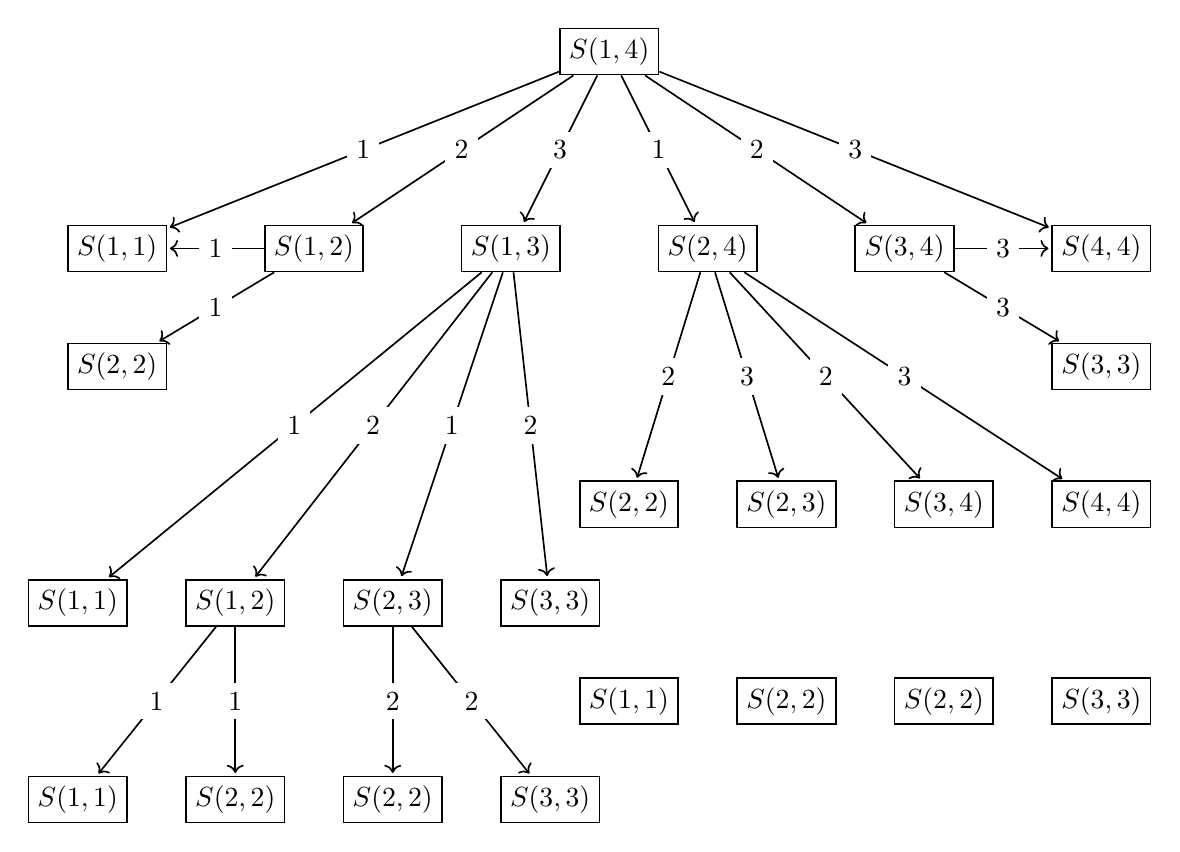
\begin{tikzpicture}[
            -{Latex}, % arrow head style
            shorten > = 1pt, % don't touch arrow head to node
            auto,
            node distance = 3cm, % distance between nodes
            semithick % line style
            ]
            \node[draw, rectangle] (1) at (1.25,0) {$S(1,4)$};
            \node[draw, rectangle] (2) at (-5, -2.5) {$S(1,1)$};
            \node[draw, rectangle] (3) at (-2.5, -2.5) {$S(1,2)$};
            \node[draw, rectangle] (4) at (0,-2.5) {$S(1,3)$};
            \node[draw, rectangle] (5) at (2.5, -2.5) {$S(2,4)$};
            \node[draw, rectangle] (6) at (5, -2.5) {$S(3,4)$};
            \node[draw, rectangle] (7) at (7.5, -2.5) {$S(4,4)$};

            \node[draw, rectangle] (8) at (-5,-4) {$S(2,2)$};
            \node[draw, rectangle] (9) at (7.5,-4) {$S(3,3)$};
            
            \node[draw, rectangle] (10) at (-5.5,-7) {$S(1,1)$};
            \node[draw, rectangle] (11) at (-3.5,-7) {$S(1,2)$};
            \node[draw, rectangle] (12) at (-1.5,-7) {$S(2,3)$};
            \node[draw, rectangle] (13) at (0.5,-7) {$S(3,3)$};
            
            \node[draw, rectangle] (14) at (1.5,-5.75) {$S(2,2)$};
            \node[draw, rectangle] (15) at (3.5,-5.75) {$S(2,3)$};
            \node[draw, rectangle] (16) at (5.5,-5.75) {$S(3,4)$};
            \node[draw, rectangle] (17) at (7.5,-5.75) {$S(4,4)$};

            \node[draw, rectangle] (18) at (-5.5,-9.5) {$S(1,1)$};
            \node[draw, rectangle] (19) at (-3.5,-9.5) {$S(2,2)$};
            \node[draw, rectangle] (20) at (-1.5,-9.5) {$S(2,2)$};
            \node[draw, rectangle] (21) at (0.5,-9.5) {$S(3,3)$};

            \node[draw, rectangle] (22) at (1.5,-8.25) {$S(1,1)$};
            \node[draw, rectangle] (23) at (3.5,-8.25) {$S(2,2)$};
            \node[draw, rectangle] (24) at (5.5,-8.25) {$S(2,2)$};
            \node[draw, rectangle] (25) at (7.5,-8.25) {$S(3,3)$};
            % \node[draw, rec]

            % \path[->] (1) edge node[midway, above]{1} (2);
            \path[->] (1) edge node[fill=white,
            anchor=center, pos=0.5] {1} (2);
            \path[->] (1) edge node[fill=white,
            anchor=center, pos=0.5] {2} (3);
            \path[->] (1) edge node[fill=white,
            anchor=center, pos=0.5] {3} (4);
            \path[->] (1) edge node[fill=white,
            anchor=center, pos=0.5] {1} (5);
            \path[->] (1) edge node[fill=white,
            anchor=center, pos=0.5] {2} (6);
            \path[->] (1) edge node[fill=white,
            anchor=center, pos=0.5] {3} (7);
            \path[->] (3) edge node[fill=white,
            anchor=center, pos=0.5] {1} (2);
            \path[->] (3) edge node[fill=white,
            anchor=center, pos=0.5] {1} (8);
            \path[->] (6) edge node[fill=white,
            anchor=center, pos=0.5] {3} (7);
            \path[->] (6) edge node[fill=white,
            anchor=center, pos=0.5] {3} (9);
            \path[->] (4) edge node[fill=white,
            anchor=center, pos=0.5] {1} (10);
            \path[->] (4) edge node[fill=white,
            anchor=center, pos=0.5] {2} (11);
            \path[->] (4) edge node[fill=white,
            anchor=center, pos=0.5] {1} (12);
            \path[->] (4) edge node[fill=white,
            anchor=center, pos=0.5] {2} (13);
            \path[->] (5) edge node[fill=white,
            anchor=center, pos=0.5] {2} (14);
            \path[->] (5) edge node[fill=white,
            anchor=center, pos=0.5] {3} (15);
            \path[->] (5) edge node[fill=white,
            anchor=center, pos=0.5] {2} (16);
            \path[->] (5) edge node[fill=white,
            anchor=center, pos=0.5] {3} (17);
            \path[->] (11) edge node[fill=white,
            anchor=center, pos=0.5] {1} (18);
            \path[->] (11) edge node[fill=white,
            anchor=center, pos=0.5] {1} (19);
            \path[->] (12) edge node[fill=white,
            anchor=center, pos=0.5] {2} (20);
            \path[->] (12) edge node[fill=white,
            anchor=center, pos=0.5] {2} (21);
            % \path[->] (3) edge node[fill=white,
            % anchor=center, pos=0.5] {1} (8);
        \end{tikzpicture}
    \end{figure}
    
    % \begin{example}
    %     Let us consider the matrix chain $A_1 \times A_2 \times A_3 \times A_4$. 
    % \end{example}

\end{document}